\documentclass[11pt,a4paper]{article}

\usepackage[margin=1in]{geometry}
\usepackage{graphicx}
\usepackage{booktabs}
\usepackage{array}
\usepackage{multirow}
\usepackage{siunitx}
\usepackage{amsmath,amssymb}
\usepackage{xcolor}
\usepackage{tikz}
\usetikzlibrary{arrows.meta,positioning,shapes.geometric,fit}
\usepackage{float}
\usepackage{placeins}
\usepackage[numbers,sort&compress]{natbib}
\usepackage[hyphens]{url}
\usepackage[colorlinks=true,linkcolor=blue,citecolor=blue,urlcolor=blue]{hyperref}

\graphicspath{{../results/figures/}{results/figures/}{figures/}}
\sisetup{round-mode=places,round-precision=3,detect-weight=true,detect-family=true}

\title{Policy-Layer Explainability for Simulated EEG-Guided Adaptive Vagus Nerve Stimulation}

\author{
Antonio Pereira\textsuperscript{1,*} \\
\textsuperscript{1}Department/Institution, City, Country \\
\textsuperscript{*}Correspondence: squareshorts@gmail.com
}

\date{}

\begin{document}
\maketitle

\begin{abstract}
Adaptive neuromodulation should be evaluated as a burden-constrained authorization policy. We studied simulated EEG-guided vagus nerve stimulation (VNS) in a CHB-MIT governance framework that converts operational risk scores into authorization windows only after calibration, persistence, and attribution-stability constraints are applied.

The analysis used five CHB-MIT scalp EEG subjects, 70 EDF files, 67.82 h of EEG, and 27 annotated seizures. Four-second overlapping windows were represented with handcrafted EEG features. Logistic regression, random forest, LightGBM, a line-length score, and prevalence baselines were evaluated with held-out-subject and within-subject chronological validation. Discrimination was moderate: LightGBM held-out-subject AUROC was $0.620 \pm 0.098$ and AUPRC was $0.142 \pm 0.062$; within-subject AUROC was $0.679 \pm 0.231$ and AUPRC was $0.269 \pm 0.203$. Nested calibration improved policy-input reliability: held-out-subject LightGBM ECE decreased from $0.211 \pm 0.081$ raw to $0.020 \pm 0.017$ after Platt scaling. In held-out-subject policy ablation, false authorization clusters decreased from $84.44 \pm 29.57$/h under fixed thresholding to $1.17 \pm 2.05$/h under the full governed policy, with fold-mean event-level authorization coverage decreasing from $1.00$ to $0.76$.

These results identify the governed authorization policy, rather than the classifier score alone, as the appropriate object of evaluation for adaptive neuromodulation simulations. Policy-layer governance converted uncertain EEG-derived scores into auditable authorization decisions and exposed the trade-off between event coverage, calibration, attribution stability, and false-intervention burden.
\end{abstract}

\noindent\textbf{Keywords:} explainable AI; EEG; adaptive neuromodulation; vagus nerve stimulation; calibration; authorization policy.

\section{Introduction}

Drug-resistant epilepsy is commonly defined as failure of adequate trials of two tolerated, appropriately chosen and used antiseizure medication schedules to achieve sustained seizure freedom\citep{kwan2010drugresistant}. For patients who remain refractory and are not candidates for curative resective surgery, neuromodulation is an important therapeutic option. Vagus nerve stimulation is used as adjunctive therapy for selected patients with refractory epilepsy, with programming shaped by dose, duty cycle, tolerability, adverse effects, battery use, and longitudinal clinical judgment\citep{morris2013vns,fahoum2022vnsparams}.

Adaptive neuromodulation changes the decision problem. Instead of using a fixed schedule alone, an adaptive system links intervention authorization to measured signals and algorithmic estimates. Contemporary VNS already includes biomarker-triggered stimulation based on ictal tachycardia\citep{fisher2016autostim}. EEG-derived estimates offer another route for adaptive triggering, but they introduce a governance problem: the system constructs an operational risk score from recorded signals, preprocessing choices, labels, model structure, calibration, and threshold rules.

This distinction is central for retrospective EEG simulation. In CHB-MIT, seizure annotations define observed ictal intervals, while preictal labels define a modeling convention around those intervals\citep{guttag2010chbmit,goldberger2000physionet}. Different preictal horizons, window lengths, feature sets, validation schemes, and thresholds produce different operational risk scores and different authorization policies. Adaptive neuromodulation should therefore be evaluated as a burden-constrained authorization policy.

AUROC is useful but incomplete for action systems. AUROC summarizes ranking across thresholds, while an authorization policy acts at specific operating points. Discrimination alone can produce high authorization burden, unstable triggering, poor calibration, or explanations that shift across adjacent windows. These properties become visible only when the model score is evaluated together with the policy that converts it into authorization windows and authorization clusters.

Explainability is also a policy-layer property. Feature attribution can show which EEG features support an operational risk score, but the present framework uses attribution stability as an authorization constraint. A governed policy can require elevated risk, temporal persistence, calibrated uncertainty, attribution stability, and burden reporting before simulated intervention authorization.

The contribution of this study is methodological. It evaluates adaptive neuromodulation as a governed authorization problem in which discrimination, calibration, temporal persistence, attribution stability, and burden are jointly measured. This provides a reproducible framework for auditing how uncertain EEG-derived scores become simulated intervention decisions.

\section{Methods}

\subsection{Framework}

The framework was implemented as a modular Python workflow with separate components for data access, windowing, feature extraction, model training, evaluation, calibration, feature attribution, policy simulation, event-level summarization, visualization, and audit tables. Configuration files defined dataset paths, windowing parameters, model choices, calibration bins, attribution-stability parameters, and policy thresholds.

\subsection{Data and Windowing}

The analysis used a real EEG subset from the CHB-MIT scalp EEG database\citep{guttag2010chbmit}. The subset included five subjects: chb01, chb02, chb03, chb05, and chb08. A total of 70 EDF recordings were analyzed, corresponding to 67.82 h of EEG and 27 annotated seizures. Recordings were sampled at 256 Hz. Duplicate channel names were harmonized, and 22 unique bipolar EEG channels were retained for feature extraction.

Continuous EEG recordings were segmented into 4 s windows with 50\% overlap. Each window was assigned a timestamp at its center. Labels were interictal, preictal, or ictal. The preictal interval was the 5 min period preceding annotated seizure onset. For binary model training and policy simulation, preictal and ictal windows were collapsed into an operational risk class; interictal windows were treated as non-risk windows.

\begin{table}[H]
\centering
\caption{Dataset summary for the five-subject CHB-MIT real-EEG subset.}
\label{tab:dataset}
\small
\begin{tabular}{lrrrr}
\toprule
Subject & EDF recordings & EEG hours & Annotated seizures & Windows \\
\midrule
chb01 & 20 & 18.55 & 7 & 33,373 \\
chb02 & 9 & 8.27 & 3 & 14,870 \\
chb03 & 13 & 13.00 & 7 & 23,387 \\
chb05 & 14 & 14.00 & 5 & 25,191 \\
chb08 & 14 & 14.00 & 5 & 25,186 \\
\midrule
Total & 70 & 67.82 & 27 & 122,007 \\
\bottomrule
\end{tabular}
\end{table}
\FloatBarrier

\subsection{Validation and Leakage Control}

Two validation modes were implemented. Held-out-subject validation used each subject as the test set in turn and trained on the remaining subjects. Within-subject chronological validation used subject-specific chronological file-level splits, with earlier recordings assigned to training and later recordings assigned to testing. No EDF file contributed windows to both training and testing.

A leakage-control audit checked train-test EDF overlap, subject overlap, held-out-subject exclusion, file-level splitting, chronological ordering in within-subject folds, and whether overlapping windows crossed a split boundary. Nested calibration used disjoint training recordings for core model fitting and calibration fitting.

\subsection{Features and Risk-Score Generators}

Each EEG window was represented with interpretable handcrafted features: amplitude summaries, line length, zero-crossing rate, Hjorth mobility, Hjorth complexity, kurtosis, spectral power, and relative band-power measures. Logistic regression, random forest, and LightGBM were evaluated as operational risk-score generators. Baseline comparisons included test-set prevalence and a simple line-length score. LightGBM was used for the main governance analysis as a representative nonlinear risk-score generator.

\subsection{Metrics and Calibration}

Window-level evaluation used AUROC, AUPRC, sensitivity, specificity, F1-score, balanced accuracy, Brier score, and false authorization windows per hour. Calibration was evaluated with 10-bin reliability curves, Brier score, expected calibration error (ECE), calibration slope, calibration intercept, maximum predicted probability, and bin counts. Platt scaling and isotonic regression were fit in a nested train-only procedure: within each outer fold, training recordings were split into core model-fitting and calibration subsets, and the outer test fold was used only for final evaluation.

\subsection{Attribution Stability}

Global explanations were generated using model-native importance measures and SHAP values for LightGBM\citep{lundberg2017shap,ke2017lightgbm}. Let $p_t$ denote the operational risk score for window $t$. Let $E_t$ denote the ranked feature-attribution set for that window and $T_k(E_t)$ the top-$k$ attributed features. Attribution stability between adjacent windows was quantified as
\[
S_t =
\frac{|T_k(E_t) \cap T_k(E_{t-1})|}
{|T_k(E_t) \cup T_k(E_{t-1})|}.
\]
The attribution-stability analysis used $k=5$. A threshold of $\gamma=0.4$ required at least three shared top-attributed features across adjacent windows.

\subsection{Governed Authorization Policies}

The governance layer formalized how operational risk scores became authorization windows. A fixed-threshold policy authorized a window when $p_t > \theta$. Temporal persistence required adjacent windows to exceed threshold. Calibration-aware gating required raw and calibrated probabilities to exceed threshold. The full governed policy required calibrated probability persistence and $S_t > \gamma$:
\[
p_t^{cal} > \theta,\qquad p_{t-1}^{cal} > \theta,\qquad S_t > \gamma.
\]
The default threshold was $\theta=0.5$ and the default stability threshold was $\gamma=0.4$.

Terminology was restricted to authorization behavior. An authorization window is a single EEG window satisfying a policy rule. An authorization cluster merges consecutive authorized windows within the same EDF recording into a single cluster. Cooldown sensitivity additionally merged authorized windows separated by 30 s, 60 s, or 120 s. The main burden metrics were authorization clusters per hour and false authorization clusters per hour. Window-level burden was retained as authorization windows per hour.

\subsection{Event-Level Authorization}

For each annotated seizure in held-out test recordings, an event was counted as covered when at least one authorization occurred from 5 min before annotated onset through annotated offset. Lead time was the negative of the first authorization latency relative to annotated onset; positive values indicate pre-onset authorization and negative values indicate first authorization after annotated onset.

\begin{figure}[H]
\centering
\resizebox{\linewidth}{!}{%
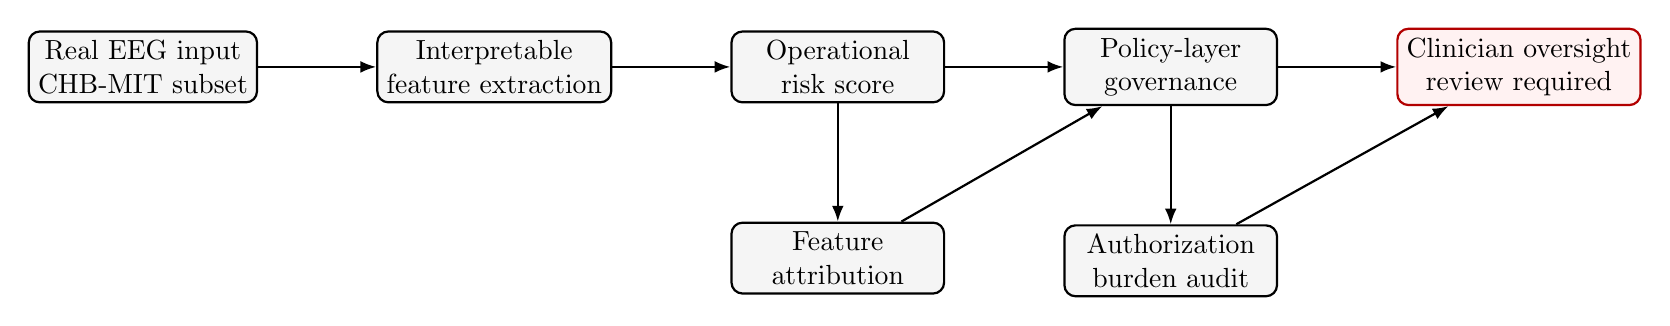
\begin{tikzpicture}[
    node distance=1.5cm,
    box/.style={rectangle, rounded corners, draw=black, thick, align=center, minimum width=2.7cm, minimum height=0.9cm, fill=gray!8},
    warn/.style={rectangle, rounded corners, draw=red!70!black, thick, align=center, minimum width=3.0cm, minimum height=0.9cm, fill=red!5},
    arrow/.style={-{Latex[length=2mm]}, thick}
]

\node[box] (eeg) {Real EEG input\\CHB-MIT subset};
\node[box, right=of eeg] (feat) {Interpretable\\feature extraction};
\node[box, right=of feat] (model) {Operational\\risk score};
\node[box, below=of model] (xai) {Feature\\attribution};
\node[box, right=of model] (policy) {Policy-layer\\governance};
\node[warn, right=of policy] (clinician) {Clinician oversight\\review required};
\node[box, below=of policy] (sim) {Authorization\\burden audit};

\draw[arrow] (eeg) -- (feat);
\draw[arrow] (feat) -- (model);
\draw[arrow] (model) -- (policy);
\draw[arrow] (policy) -- (clinician);
\draw[arrow] (model) -- (xai);
\draw[arrow] (xai) -- (policy);
\draw[arrow] (policy) -- (sim);
\draw[arrow] (sim) -- (clinician);
\end{tikzpicture}
}
\caption{Governed adaptive neuromodulation pipeline. EEG windows are converted into interpretable features, scored for operational risk, explained through feature attribution, and passed to policy-layer governance. The output is an auditable authorization burden profile.}
\label{fig:pipeline}
\end{figure}
\FloatBarrier

\section{Results}

\subsection{Cohort and Leakage Audit}

The five-subject CHB-MIT subset contained 70 EDF recordings, 67.82 h of EEG, and 27 annotated seizures. Sliding-window segmentation produced 122,007 windows. Held-out-subject evaluation contained 5,227 positive operational-risk windows across the five test folds. Within-subject chronological evaluation contained 49,564 held-out test windows, including 1,986 positive operational-risk windows.

The leakage-control audit found no EDF overlap between train and test sets in any evaluation fold. Held-out-subject folds had zero subject overlap between train and test sets, and the held-out subject was absent from training in all five folds. Within-subject folds had subject overlap by design, used chronological file-level splits, and had no overlapping windows crossing train-test boundaries.

\begin{table}[H]
\centering
\caption{Leakage-control audit summary. Values summarize fold-level split checks.}
\label{tab:leakage_audit}
\small
\resizebox{\linewidth}{!}{
\begin{tabular}{lrrrr}
\toprule
Validation mode & Folds & Train-test EDF overlap & Held-out subject in train & File-level split \\
\midrule
Held-out subject & 5 & 0/5 & 0/5 & 5/5 \\
Within-subject chronological & 5 & 0/5 & Not applicable & 5/5 \\
\bottomrule
\end{tabular}
}
\end{table}
\FloatBarrier

\subsection{Baseline Discrimination Establishes the Risk-Score Setting}

Model discrimination was moderate (Table~\ref{tab:performance}, Figure~\ref{fig:performance}). Held-out-subject LightGBM AUROC was $0.620 \pm 0.098$ and AUPRC was $0.142 \pm 0.062$. The line-length baseline had similar held-out-subject AUROC ($0.616 \pm 0.136$), and logistic regression had higher held-out-subject AUPRC ($0.159 \pm 0.115$) than LightGBM. Within-subject validation showed higher but variable performance.

The baseline comparison indicates that the predictive model should be treated as a risk-score generator rather than as the primary contribution. The main analysis therefore focuses on how governance constraints alter the translation from risk scores to intervention authorization.

\begin{table}[H]
\centering
\caption{Window-level operational-risk discrimination and thresholded classification summaries. Values are mean $\pm$ standard deviation across five folds.}
\label{tab:performance}
\scriptsize
\resizebox{\linewidth}{!}{
\begin{tabular}{llrrrrrrr}
\toprule
Validation mode & Model & AUROC & AUPRC & Sens. & Spec. & F1 & Bal. acc. & False auth. windows/h \\
\midrule
Held-out subject & Logistic regression & $0.551 \pm 0.114$ & $0.159 \pm 0.115$ & $0.358 \pm 0.167$ & $0.764 \pm 0.160$ & $0.114 \pm 0.053$ & $0.561 \pm 0.063$ & $407.83 \pm 279.79$ \\
Held-out subject & Random forest & $0.597 \pm 0.037$ & $0.124 \pm 0.064$ & $0.058 \pm 0.046$ & $0.995 \pm 0.010$ & $0.095 \pm 0.076$ & $0.527 \pm 0.022$ & $9.08 \pm 18.01$ \\
Held-out subject & LightGBM & $0.620 \pm 0.098$ & $0.142 \pm 0.062$ & $0.328 \pm 0.145$ & $0.853 \pm 0.064$ & $0.137 \pm 0.041$ & $0.591 \pm 0.048$ & $254.44 \pm 112.52$ \\
\midrule
Within-subject chronological & Logistic regression & $0.659 \pm 0.240$ & $0.197 \pm 0.150$ & $0.572 \pm 0.245$ & $0.676 \pm 0.137$ & $0.135 \pm 0.081$ & $0.624 \pm 0.185$ & $560.05 \pm 239.66$ \\
Within-subject chronological & Random forest & $0.660 \pm 0.229$ & $0.267 \pm 0.204$ & $0.174 \pm 0.147$ & $0.996 \pm 0.002$ & $0.258 \pm 0.204$ & $0.585 \pm 0.074$ & $6.50 \pm 3.83$ \\
Within-subject chronological & LightGBM & $0.679 \pm 0.231$ & $0.269 \pm 0.203$ & $0.295 \pm 0.224$ & $0.928 \pm 0.023$ & $0.195 \pm 0.154$ & $0.611 \pm 0.121$ & $123.94 \pm 37.73$ \\
\bottomrule
\end{tabular}
}
\end{table}

\begin{figure}[H]
\centering

\includegraphics[width=0.98\linewidth]{figure2_model_performance_real_eeg.png}
\caption{AUROC and AUPRC across validation modes. Bars show fold means with standard-deviation error bars for logistic regression, random forest, LightGBM, and the line-length baseline. Dashed references show chance AUROC and prevalence AUPRC.}
\label{fig:performance}
\end{figure}
\FloatBarrier

\subsection{Nested Calibration Improves Policy-Input Reliability}

Nested calibration improved the numerical reliability of LightGBM policy inputs (Table~\ref{tab:calibration}, Figure~\ref{fig:calibration}). In held-out-subject validation, ECE decreased from $0.211 \pm 0.081$ raw to $0.020 \pm 0.017$ after Platt scaling and $0.021 \pm 0.018$ after isotonic calibration. Brier score decreased from $0.127 \pm 0.037$ raw to approximately $0.040$ after calibration. Within-subject validation showed a similar ECE decrease from $0.065 \pm 0.030$ raw to $0.032 \pm 0.018$ with Platt scaling and $0.026 \pm 0.020$ with isotonic calibration.

Calibration improved the numerical reliability of policy inputs but did not improve discrimination. Platt scaling preserved ranking metrics, while isotonic calibration slightly changed AUROC and AUPRC in both validation modes.

\begin{table}[H]
\centering
\caption{Nested train-only calibration diagnostics for LightGBM operational risk scores. Values are mean $\pm$ standard deviation across five folds.}
\label{tab:calibration}
\scriptsize
\resizebox{\linewidth}{!}{
\begin{tabular}{llrrrrrrr}
\toprule
Validation mode & Calibration & AUROC & AUPRC & Brier & ECE & Slope & Intercept & Max $p$ \\
\midrule
Held-out subject & Raw & $0.612 \pm 0.053$ & $0.133 \pm 0.053$ & $0.127 \pm 0.037$ & $0.211 \pm 0.081$ & $0.353 \pm 0.174$ & $-2.747 \pm 0.373$ & $0.990 \pm 0.005$ \\
Held-out subject & Platt & $0.612 \pm 0.053$ & $0.133 \pm 0.053$ & $0.040 \pm 0.009$ & $0.020 \pm 0.017$ & $0.820 \pm 0.498$ & $-0.171 \pm 1.595$ & $0.315 \pm 0.161$ \\
Held-out subject & Isotonic & $0.600 \pm 0.042$ & $0.120 \pm 0.046$ & $0.041 \pm 0.010$ & $0.021 \pm 0.018$ & $0.995 \pm 0.956$ & $0.410 \pm 3.413$ & $1.000 \pm 0.000$ \\
\midrule
Within-subject chronological & Raw & $0.712 \pm 0.230$ & $0.283 \pm 0.210$ & $0.058 \pm 0.027$ & $0.065 \pm 0.030$ & $0.280 \pm 0.301$ & $-2.369 \pm 1.007$ & $0.998 \pm 0.003$ \\
Within-subject chronological & Platt & $0.712 \pm 0.230$ & $0.283 \pm 0.210$ & $0.036 \pm 0.019$ & $0.032 \pm 0.018$ & $1.189 \pm 1.470$ & $-0.162 \pm 3.646$ & $0.586 \pm 0.249$ \\
Within-subject chronological & Isotonic & $0.682 \pm 0.190$ & $0.218 \pm 0.155$ & $0.036 \pm 0.020$ & $0.026 \pm 0.020$ & $0.255 \pm 0.376$ & $-2.488 \pm 1.401$ & $1.000 \pm 0.000$ \\
\bottomrule
\end{tabular}
}
\end{table}

\begin{figure}[H]
\centering
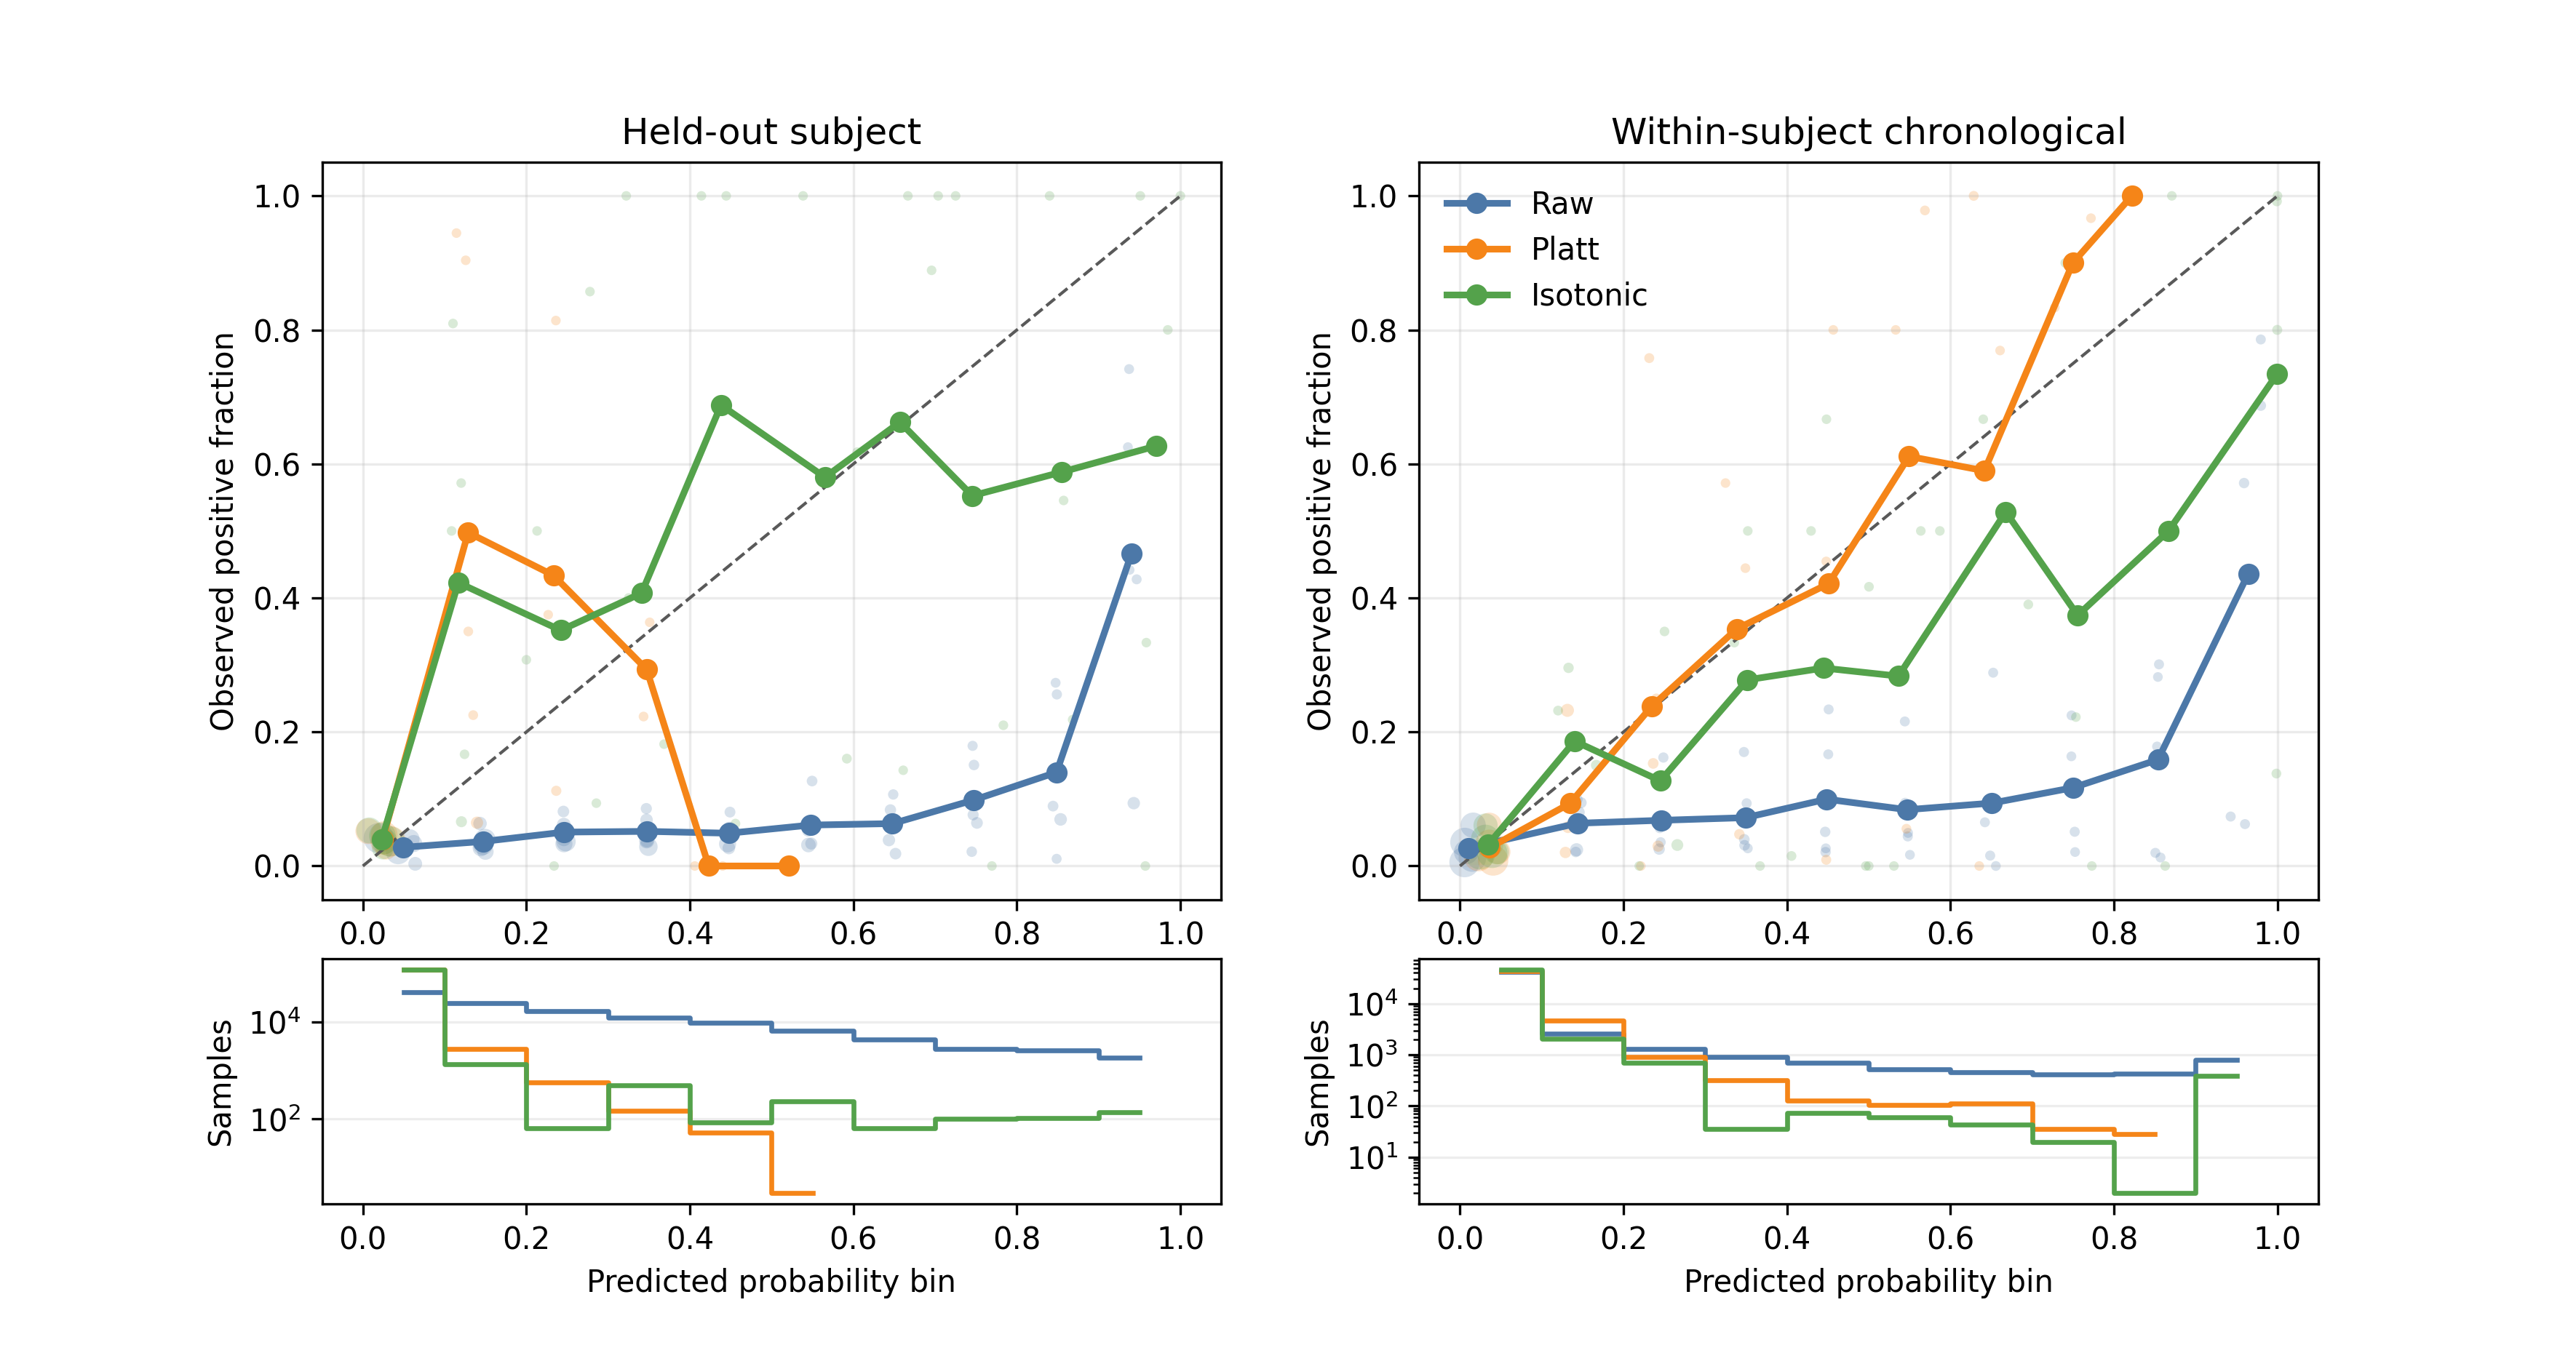
\includegraphics[width=0.98\linewidth]{figure3_calibration_diagnostics_real_eeg.png}
\caption{Nested calibration diagnostics for LightGBM. Reliability curves compare raw, Platt-scaled, and isotonic probabilities; marker size reflects bin count, and lower panels show predicted-probability bin counts on a log scale.}
\label{fig:calibration}
\end{figure}
\FloatBarrier

\subsection{Policy Ablation Reduces Authorization Burden}

The policy ablation identified the governance layer as the main determinant of burden (Table~\ref{tab:operating}). In held-out-subject validation, fixed thresholding produced $270.05 \pm 118.01$ authorization windows/h and $88.38 \pm 30.05$ authorization clusters/h. Adding temporal persistence reduced false authorization clusters from $84.44 \pm 29.57$/h to $46.01 \pm 16.69$/h. Calibration-aware gating reduced false authorization clusters to $2.70 \pm 4.60$/h. The full governed policy reduced false authorization clusters to $1.17 \pm 2.05$/h and increased mean authorized-window $S_t$ from $0.578 \pm 0.047$ to $0.834 \pm 0.083$.

The coverage-burden trade-off was explicit. Held-out-subject fold-mean event-level authorization coverage decreased from $1.00$ under fixed thresholding to $0.76 \pm 0.29$ under the full governed policy. Positive authorization rate increased from $0.093$ to $0.703$, indicating that governed authorizations were more concentrated in operational-risk windows.

\begin{table}[H]
\centering
\caption{Selected LightGBM operating points. Values are mean $\pm$ standard deviation across five folds. Authorization clusters merge consecutive authorized windows; cooldown sensitivity is reported separately.}
\label{tab:operating}
\scriptsize
\resizebox{\linewidth}{!}{
\begin{tabular}{llrllrrrrrrr}
\toprule
Validation mode & Policy & $\theta$ & Calibration & Persist. & $S_t$ gate & Auth. windows/h & Auth. clusters/h & False clusters/h & Coverage & Median lead (s) & Mean $S_t$ \\
\midrule
Within-subject chronological & Fixed threshold & 0.5 & raw & 1 & -- & $95.99 \pm 19.18$ & $44.11 \pm 8.84$ & $40.37 \pm 10.51$ & $1.00 \pm 0.00$ & $259.5 \pm 49.9$ & $0.665 \pm 0.048$ \\
Within-subject chronological & Threshold + temporal persistence & 0.5 & raw & 2 & -- & $45.11 \pm 16.75$ & $18.06 \pm 5.39$ & $15.67 \pm 5.43$ & $1.00 \pm 0.00$ & $155.3 \pm 149.4$ & $0.771 \pm 0.064$ \\
Within-subject chronological & Threshold + attribution-stability gate & 0.5 & raw & 1 & 0.4 & $89.87 \pm 17.96$ & $41.50 \pm 6.80$ & $37.87 \pm 8.52$ & $1.00 \pm 0.00$ & $245.3 \pm 79.0$ & $0.694 \pm 0.043$ \\
Within-subject chronological & Threshold + calibration-aware gate & 0.5 & raw + isotonic & 1 & -- & $15.92 \pm 10.42$ & $4.82 \pm 2.41$ & $3.53 \pm 1.96$ & $1.00 \pm 0.00$ & $72.1 \pm 105.3$ & $0.772 \pm 0.085$ \\
Within-subject chronological & Full governed policy & 0.5 & isotonic & 2 & 0.4 & $10.38 \pm 9.28$ & $1.67 \pm 0.92$ & $0.95 \pm 0.80$ & $0.93 \pm 0.15$ & $26.1 \pm 92.5$ & $0.846 \pm 0.073$ \\
\midrule
Held-out subject & Fixed threshold & 0.5 & raw & 1 & -- & $270.05 \pm 118.01$ & $88.38 \pm 30.05$ & $84.44 \pm 29.57$ & $1.00 \pm 0.00$ & $235.8 \pm 60.7$ & $0.578 \pm 0.047$ \\
Held-out subject & Threshold + temporal persistence & 0.5 & raw & 2 & -- & $160.82 \pm 101.90$ & $49.14 \pm 16.77$ & $46.01 \pm 16.69$ & $1.00 \pm 0.00$ & $184.0 \pm 113.5$ & $0.658 \pm 0.049$ \\
Held-out subject & Threshold + attribution-stability gate & 0.5 & raw & 1 & 0.4 & $229.33 \pm 104.79$ & $79.18 \pm 26.55$ & $75.23 \pm 26.26$ & $1.00 \pm 0.00$ & $234.6 \pm 61.3$ & $0.642 \pm 0.041$ \\
Held-out subject & Threshold + calibration-aware gate & 0.5 & raw + isotonic & 1 & -- & $10.01 \pm 13.77$ & $3.31 \pm 4.67$ & $2.70 \pm 4.60$ & $0.76 \pm 0.29$ & $7.7 \pm 57.5$ & $0.739 \pm 0.101$ \\
Held-out subject & Full governed policy & 0.5 & isotonic & 2 & 0.4 & $5.80 \pm 7.76$ & $1.72 \pm 2.10$ & $1.17 \pm 2.05$ & $0.76 \pm 0.29$ & $-17.4 \pm 10.8$ & $0.834 \pm 0.083$ \\
\bottomrule
\end{tabular}
}
\end{table}
\FloatBarrier

\subsection{Burden-Constrained Operating Curves Expose Coverage-Burden Trade-Offs}

Held-out-subject sweeps showed that no single threshold dominated across objectives (Figure~\ref{fig:operating_curves}). Lower thresholds increased event-level authorization coverage but increased false authorization clusters. Higher thresholds and governed policies moved the operating point into a lower-burden region while reducing coverage. The selected governed region reduced false authorization burden while preserving partial event-level coverage.

\begin{figure}[H]
\centering
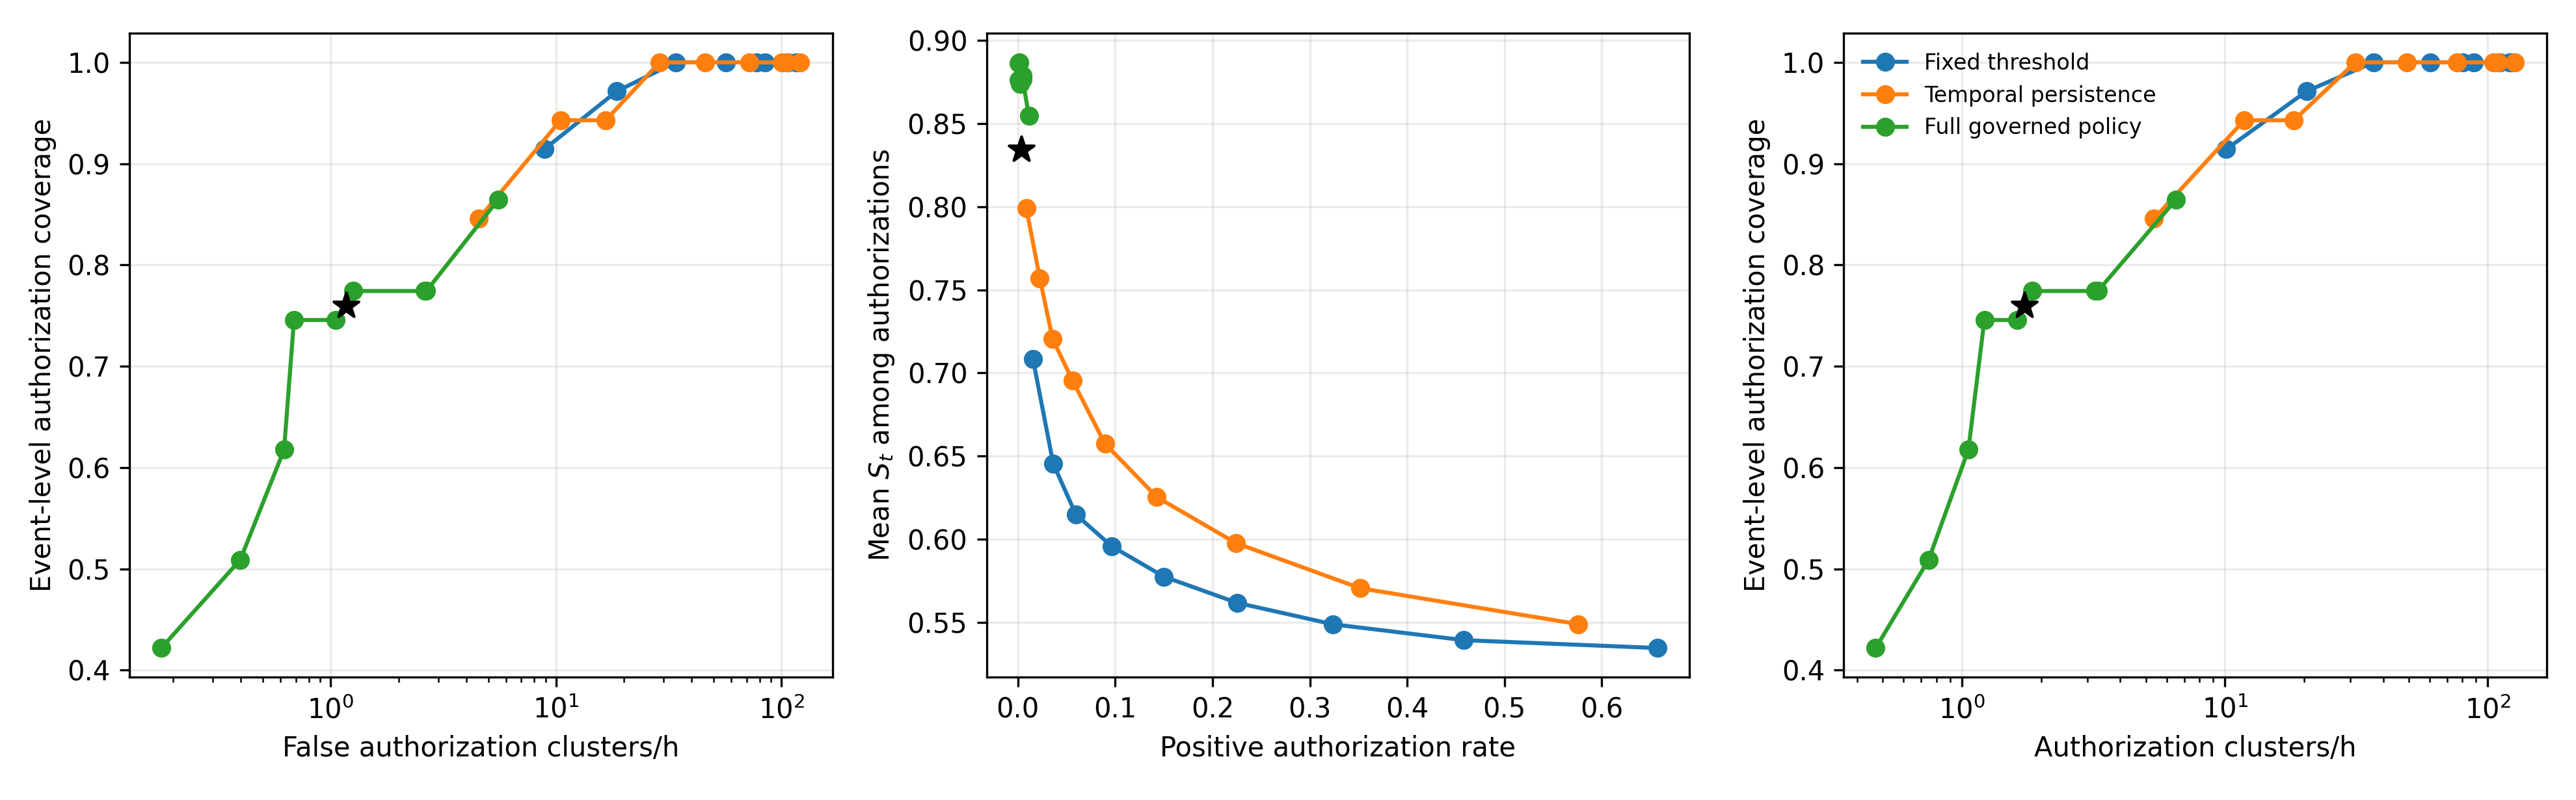
\includegraphics[width=0.98\linewidth]{figure5_burden_constrained_operating_curves_real_eeg.png}
\caption{Burden-constrained operating curves for held-out-subject policy sweeps. Curves show the trade-off between event-level authorization coverage, authorization burden, and attribution stability across threshold and governance-parameter settings. The selected governed operating region reduces false authorization burden while preserving partial event-level coverage.}
\label{fig:operating_curves}
\end{figure}
\FloatBarrier

\subsection{Attribution-Stability Gating Adds Evidence Consistency}

Attribution-stability gating reduced false authorization burden and increased evidence consistency (Figure~\ref{fig:stability}, Table~\ref{tab:stability_diag}). In held-out-subject validation, false authorization clusters decreased from $84.44 \pm 29.57$/h under fixed thresholding to $75.23 \pm 26.26$/h with an attribution-stability gate, and mean authorized-window $S_t$ increased from $0.578 \pm 0.047$ to $0.642 \pm 0.041$. Among fixed-threshold authorization windows, true authorizations had higher mean $S_t$ than false authorizations in both validation modes.

The probability-stability relationship was weak. Mean Spearman correlation between $p_t$ and $S_t$ was $-0.053 \pm 0.137$ in held-out-subject validation and $-0.077 \pm 0.125$ in within-subject validation, supporting attribution stability as a distinct governance signal.

\begin{figure}[H]
\centering
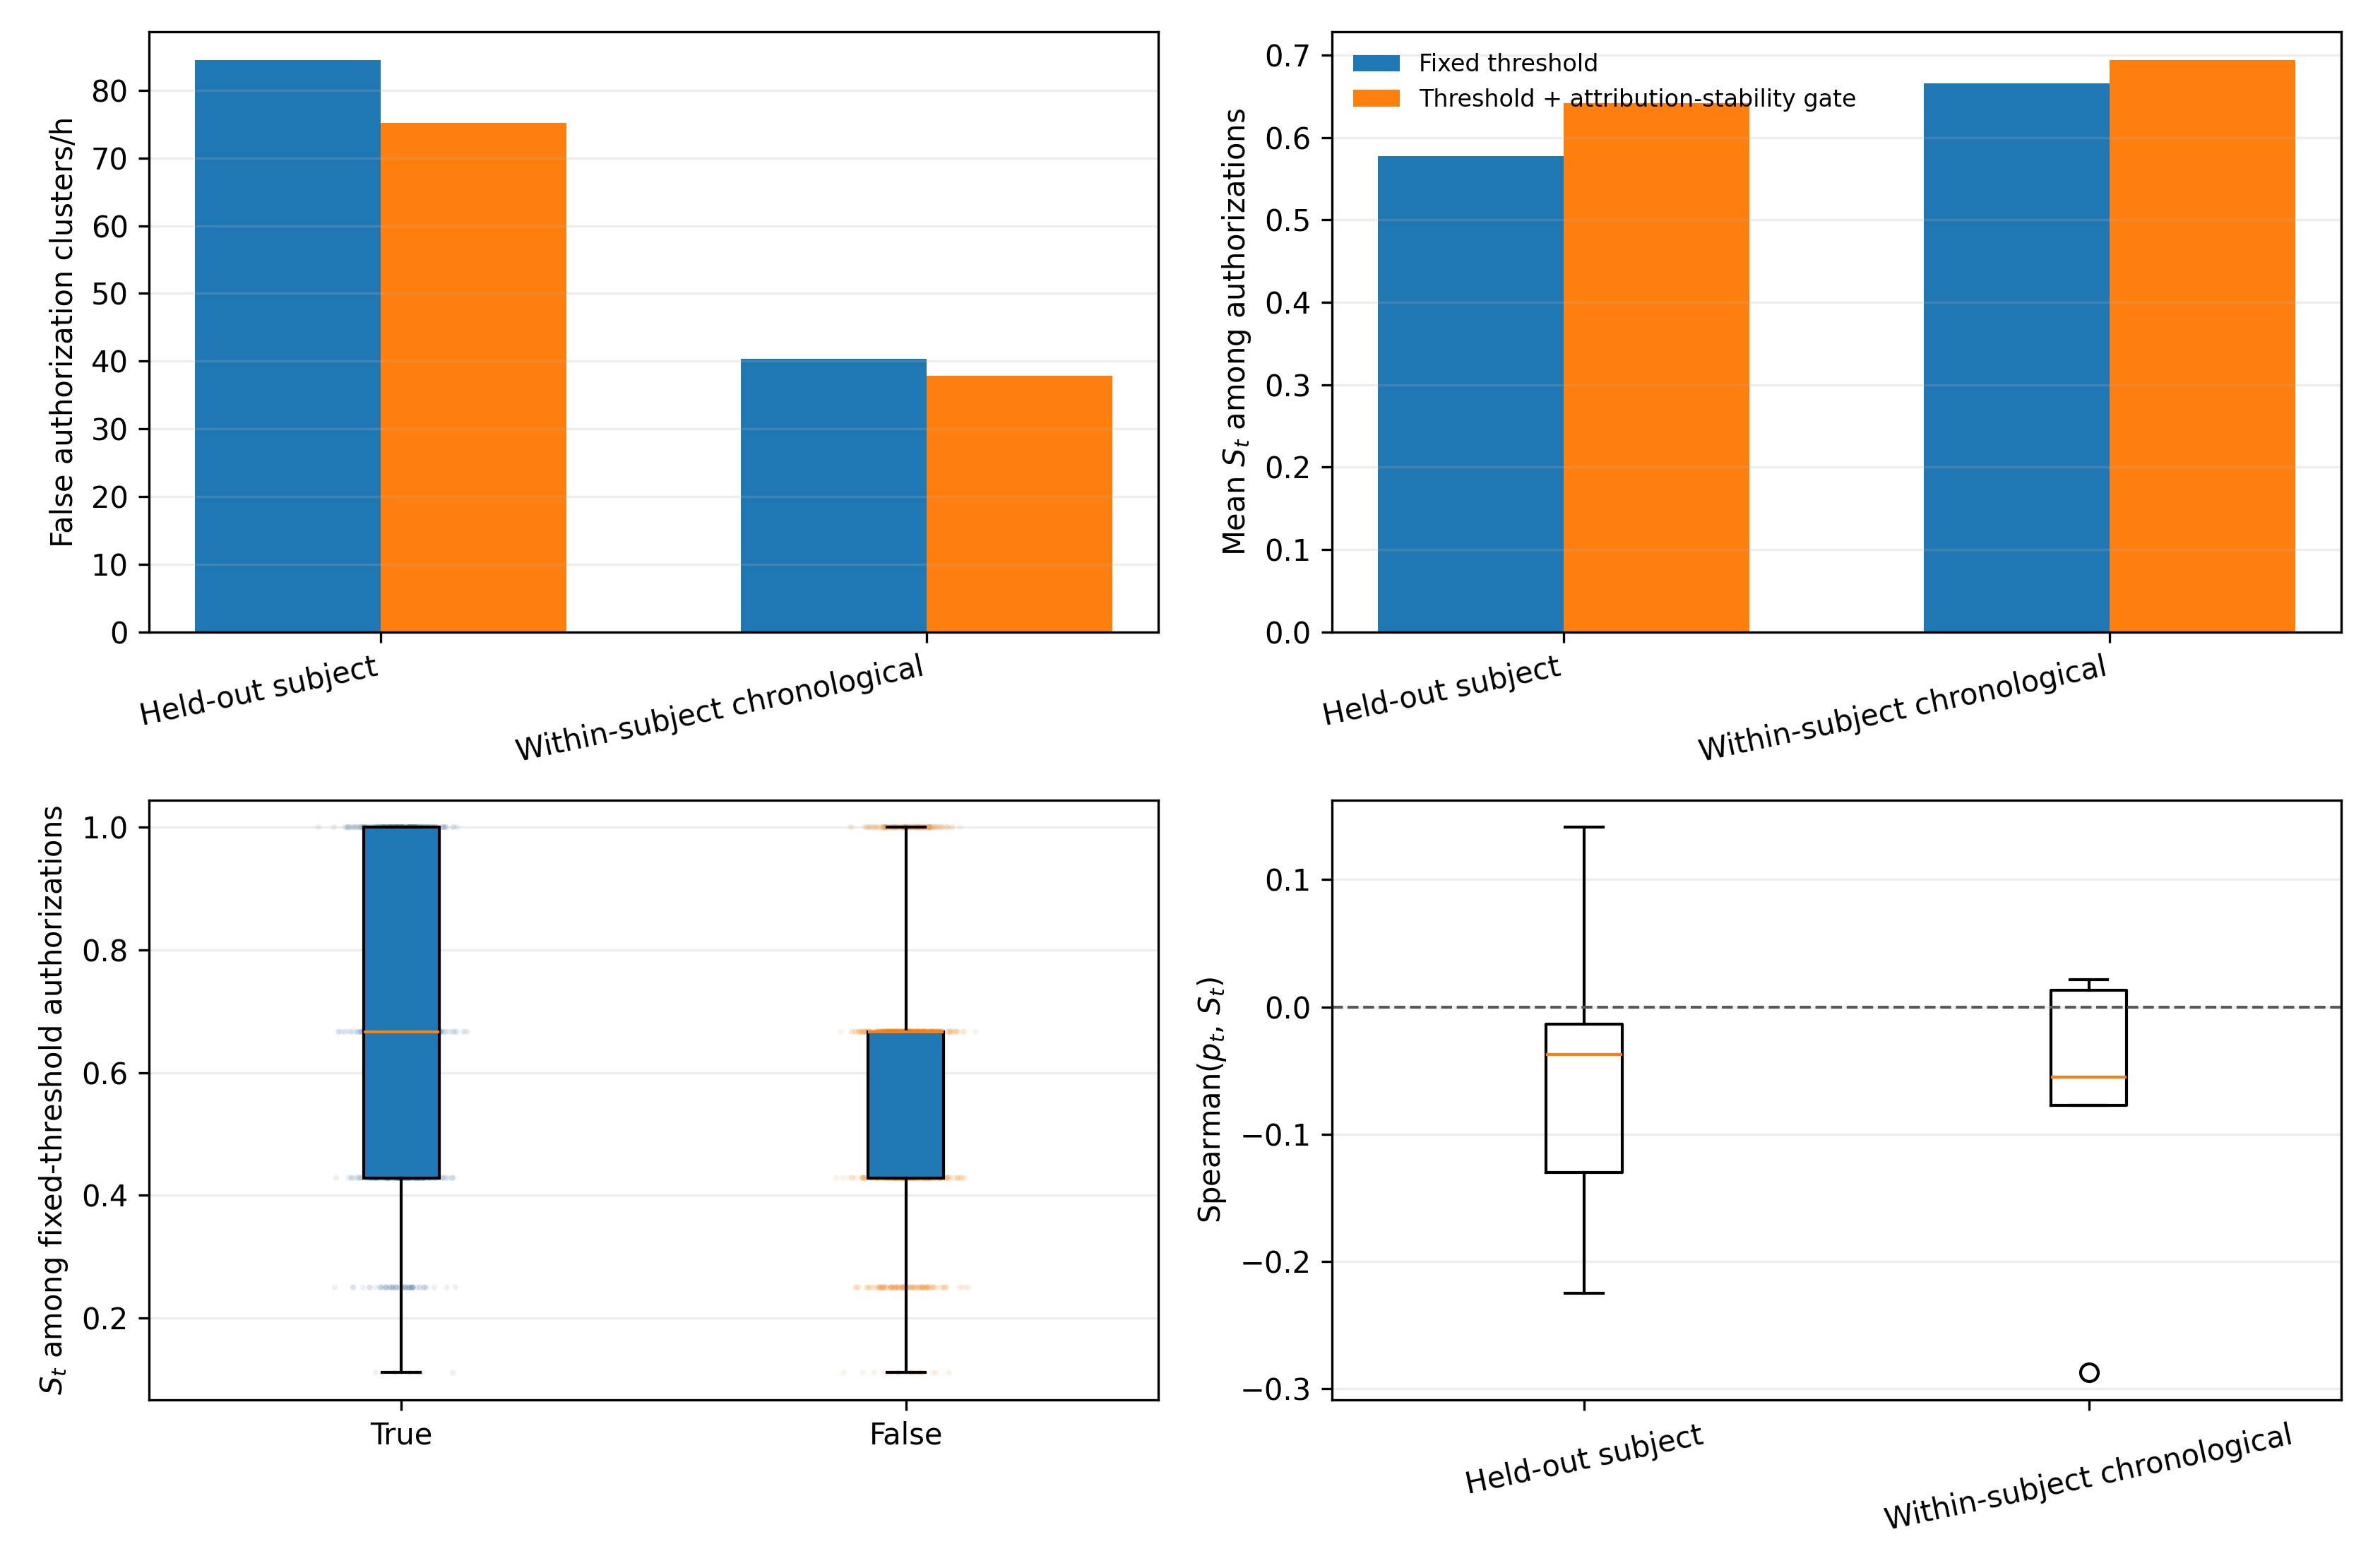
\includegraphics[width=0.98\linewidth]{figure4_attribution_stability_governance_real_eeg.png}
\caption{Attribution-stability governance diagnostics. Panels show false authorization clusters before and after stability gating, mean $S_t$ before and after gating, $S_t$ distributions for true and false fixed-threshold authorizations, and the fold-level Spearman relationship between probability and attribution stability.}
\label{fig:stability}
\end{figure}

\begin{table}[H]
\centering
\caption{Relationship between LightGBM probability and attribution stability. Values are mean $\pm$ standard deviation across five folds.}
\label{tab:stability_diag}
\small
\resizebox{\linewidth}{!}{
\begin{tabular}{lrrrrr}
\toprule
Validation mode & Spearman($p_t,S_t$) & True auth. $S_t$ & False auth. $S_t$ & True auth. $p_t$ & False auth. $p_t$ \\
\midrule
Held-out subject & $-0.053 \pm 0.137$ & $0.658 \pm 0.048$ & $0.569 \pm 0.050$ & $0.762 \pm 0.042$ & $0.666 \pm 0.062$ \\
Within-subject chronological & $-0.077 \pm 0.125$ & $0.710 \pm 0.135$ & $0.639 \pm 0.032$ & $0.871 \pm 0.064$ & $0.740 \pm 0.048$ \\
\bottomrule
\end{tabular}
}
\end{table}
\FloatBarrier

\subsection{Event-Level Authorization Summaries}

Event-level summaries showed how window policies mapped to annotated seizures (Table~\ref{tab:event_level}). In held-out-subject validation, fixed thresholding covered 27/27 events and the full governed policy covered 19/27 events. Fold-mean event-level authorization coverage decreased from $1.00$ to $0.76 \pm 0.29$ while false authorization clusters decreased from $84.44 \pm 29.57$/h to $1.17 \pm 2.05$/h. Pre-onset authorization counts also decreased, reflecting the burden-coverage trade-off introduced by calibration-aware persistence and attribution-stability constraints.

\begin{table}[H]
\centering
\caption{Event-level authorization summaries for LightGBM policies. Coverage is reported both as pooled event counts and as fold-mean coverage.}
\label{tab:event_level}
\scriptsize
\resizebox{\linewidth}{!}{
\begin{tabular}{llrrrrr}
\toprule
Validation mode & Policy & Events covered & Pre-onset auth. & Fold coverage & Median lead (s) & False clusters/h \\
\midrule
Within-subject chronological & Fixed threshold & 10/10 & 10 & $1.00 \pm 0.00$ & $259.5 \pm 49.9$ & $40.37 \pm 10.51$ \\
Within-subject chronological & Threshold + temporal persistence & 10/10 & 7 & $1.00 \pm 0.00$ & $155.3 \pm 149.4$ & $15.67 \pm 5.43$ \\
Within-subject chronological & Threshold + attribution-stability gate & 10/10 & 9 & $1.00 \pm 0.00$ & $245.3 \pm 79.0$ & $37.87 \pm 8.52$ \\
Within-subject chronological & Threshold + calibration-aware gate & 10/10 & 4 & $1.00 \pm 0.00$ & $72.1 \pm 105.3$ & $3.53 \pm 1.96$ \\
Within-subject chronological & Full governed policy & 9/10 & 2 & $0.93 \pm 0.15$ & $26.1 \pm 92.5$ & $0.95 \pm 0.80$ \\
\midrule
Held-out subject & Fixed threshold & 27/27 & 24 & $1.00 \pm 0.00$ & $235.8 \pm 60.7$ & $84.44 \pm 29.57$ \\
Held-out subject & Threshold + temporal persistence & 27/27 & 22 & $1.00 \pm 0.00$ & $184.0 \pm 113.5$ & $46.01 \pm 16.69$ \\
Held-out subject & Threshold + attribution-stability gate & 27/27 & 23 & $1.00 \pm 0.00$ & $234.6 \pm 61.3$ & $75.23 \pm 26.26$ \\
Held-out subject & Threshold + calibration-aware gate & 19/27 & 3 & $0.76 \pm 0.29$ & $7.7 \pm 57.5$ & $2.70 \pm 4.60$ \\
Held-out subject & Full governed policy & 19/27 & 1 & $0.76 \pm 0.29$ & $-17.4 \pm 10.8$ & $1.17 \pm 2.05$ \\
\bottomrule
\end{tabular}
}
\end{table}
\FloatBarrier

\section{Discussion}

The main finding is that adaptive neuromodulation simulations are governed by the authorization policy more than by the classifier score alone. In this CHB-MIT simulation, fixed-threshold authorization produced high burden, while calibration-aware persistence and stable-attribution constraints shifted LightGBM operating points toward lower false authorization cluster rates and higher evidence consistency.

AUROC is insufficient for action systems because it does not specify how often an intervention would be authorized. The line-length baseline achieved similar held-out-subject AUROC to LightGBM, and logistic regression achieved higher held-out-subject AUPRC. The discriminative model is therefore best interpreted as an operational risk-score generator. The clinically relevant analysis is how a score becomes an authorization window, how windows merge into clusters, and how false authorization burden changes across operating points.

Calibration acts as policy-input governance. Raw LightGBM scores were overconfident in reliability diagrams, while nested Platt and isotonic calibration improved Brier score and ECE. Calibration changed the numerical interpretation of risk thresholds used by the governance layer. It did not change the underlying event labels or provide new discrimination; it made the policy input more auditable.

Attribution stability adds an evidence-consistency constraint. A policy that authorizes an intervention from a single high score may act on transient or unstable evidence. Requiring top-feature overlap across adjacent windows suppresses part of that unstable authorization pattern and produces a measurable $S_t$ profile for the authorized windows. The weak probability-$S_t$ correlation indicates that stability contributes information not captured by the risk score alone.

The burden/event-coverage trade-off is the central operating result. Held-out-subject fixed thresholding covered all annotated events but generated $84.44 \pm 29.57$ false authorization clusters/h. The full governed policy reduced this to $1.17 \pm 2.05$ false authorization clusters/h while fold-mean event-level coverage decreased to $0.76 \pm 0.29$. This trade-off is exactly what a burden-constrained authorization analysis is designed to expose.

For adaptive neuromodulation research, these results motivate evaluating governed authorization policies rather than isolated risk scores. Future systems should report discrimination, calibration, authorization windows, authorization clusters, false authorization burden, event-level coverage, attribution stability, and operating-point selection together. This framework gives reviewers and clinicians an auditable map from uncertain EEG-derived scores to simulated intervention decisions.

\section{Limitations}

This study used a five-subject CHB-MIT subset, pediatric scalp EEG, retrospective annotations, and a fixed 5 min preictal labeling convention. The operational risk class combined preictal and ictal windows. These choices determine the simulated authorization target and should not be treated as a physiological ground truth.

The analysis evaluates simulated authorization policies, not delivered VNS therapy. It does not model stimulation dose, duty cycle, battery state, adverse effects, seizure termination, or longitudinal response.

The attribution-stability rule uses top-feature overlap across adjacent windows. External validation is required across larger cohorts, adult datasets, different montages, seizure types, and device constraints.

\section{Future Work}

Future work should expand the cohort, evaluate external EEG datasets, compare preictal labeling horizons, and test policy selection under prespecified burden constraints. Prospective extensions would require time-stamped device data, delivered therapy parameters, adverse effects, and longitudinal seizure outcomes.

\section{Conclusion}

This study presents a policy-layer explainability framework for simulated EEG-guided adaptive VNS. The analysis treats operational risk scores as inputs to governed authorization policies. Across five CHB-MIT subjects, calibration-aware persistence and attribution-stability constraints reduced false authorization clusters while exposing the cost in event-level coverage. The appropriate object of evaluation is the governed policy that converts uncertain EEG-derived scores into auditable authorization decisions.

\section*{Data and Code Availability}

The analysis uses the CHB-MIT scalp EEG database, available through PhysioNet\citep{guttag2010chbmit,goldberger2000physionet}. Analysis scripts, configuration files, generated CSV tables, and regenerated figures are organized in the project repository for reproducibility.

\section*{Ethics Statement}

The analysis used de-identified public EEG data from PhysioNet and did not involve direct interaction with human participants. Any extension to local clinical cohorts would require institutional review and appropriate governance for clinical AI research.

\section*{Author Contributions}

Antonio Pereira conceptualized the study, specified the clinical and ethical constraints, supervised the computational framing, and prepared the manuscript. Additional contributors should be added according to their roles in coding, validation, data curation, and manuscript revision.

\section*{Conflict of Interest}

The author declares no conflict of interest. This statement should be updated before submission if any author has financial, clinical, or device-related conflicts relevant to VNS, epilepsy care, or AI decision support.

\section*{Funding}

No specific funding was reported for the present work. This statement should be updated before submission.

\section*{Acknowledgments}

The author acknowledges the developers and maintainers of open-source scientific Python tools and the PhysioNet contributors who maintain public physiological signal resources.

\appendix
\section{Cooldown Sensitivity}

Table~\ref{tab:cooldown} summarizes the held-out-subject cluster burden for consecutive-window clusters and 30 s, 60 s, and 120 s cooldown alternatives.

\begin{table}[H]
\centering
\caption{Held-out-subject cooldown sensitivity for LightGBM fixed-threshold and full governed policies. Values are mean $\pm$ standard deviation across five folds.}
\label{tab:cooldown}
\small
\resizebox{\linewidth}{!}{
\begin{tabular}{llrrrr}
\toprule
Policy & Cooldown (s) & Auth. clusters/h & False clusters/h & Median duration (s) & Coverage \\
\midrule
Fixed threshold & 0 & $88.38 \pm 30.05$ & $84.44 \pm 29.57$ & $4.8 \pm 1.1$ & $1.00 \pm 0.00$ \\
Fixed threshold & 30 & $20.42 \pm 4.10$ & $19.49 \pm 4.10$ & $22.0 \pm 7.9$ & $1.00 \pm 0.00$ \\
Fixed threshold & 60 & $10.42 \pm 1.36$ & $9.79 \pm 1.39$ & $51.6 \pm 15.5$ & $1.00 \pm 0.00$ \\
Fixed threshold & 120 & $5.11 \pm 0.92$ & $4.67 \pm 0.82$ & $184.4 \pm 94.0$ & $1.00 \pm 0.00$ \\
\midrule
Full governed policy & 0 & $1.72 \pm 2.10$ & $1.17 \pm 2.05$ & $5.2 \pm 1.1$ & $0.76 \pm 0.29$ \\
Full governed policy & 30 & $1.10 \pm 1.20$ & $0.76 \pm 1.15$ & $7.8 \pm 5.8$ & $0.76 \pm 0.29$ \\
Full governed policy & 60 & $0.97 \pm 1.01$ & $0.64 \pm 0.95$ & $8.4 \pm 5.7$ & $0.76 \pm 0.29$ \\
Full governed policy & 120 & $0.86 \pm 0.82$ & $0.56 \pm 0.77$ & $13.2 \pm 9.2$ & $0.76 \pm 0.29$ \\
\bottomrule
\end{tabular}
}
\end{table}

\bibliographystyle{plainnat}
\bibliography{references}

\end{document}
